\section{REFRACCIÓN}
\subsection{Concepto}

\begin{frame}{REFRACCIÓN}
  \framesubtitle{Concepto}
  \begin{itemize}
    \item Cuando una onda electromagnética pasa de una medio a otro, se desvía respecto al ángulo incidente.
    \item Puede ocurrir al mismo tiempo que la reflexión\footnote{\bibentry{sears}}.
  \end{itemize}
  \begin{figure}
      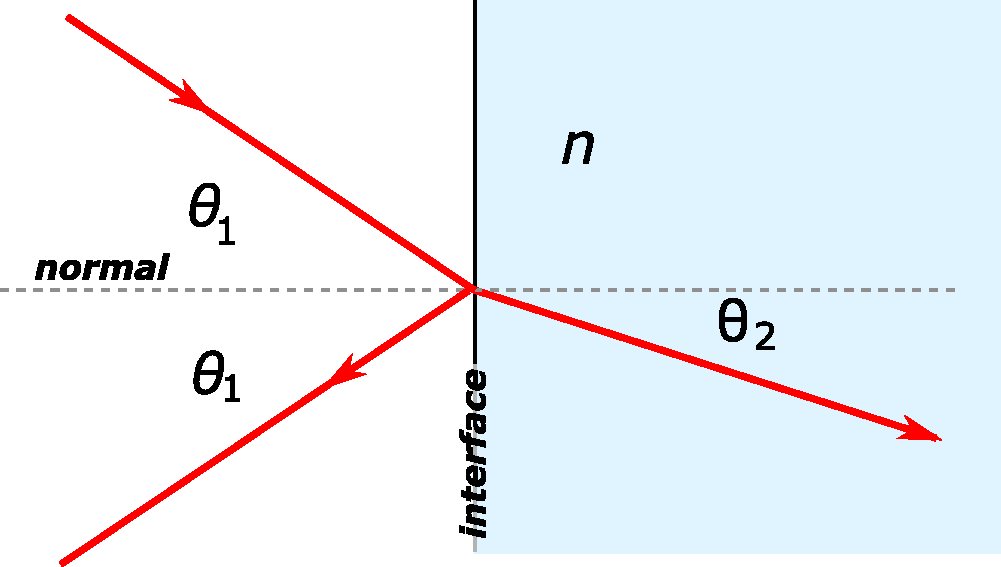
\includegraphics[scale=0.4]{david/Refrac.pdf}
      \caption{Reflexión y refracción\footnotemark{}.}
  \end{figure}
  \vspace{-2cm}\footnotetext{\bibentry{refrac}}
\end{frame}

\subsection{Índice de Refracción}

\begin{frame}{REFRACCIÓN}
  \framesubtitle{Índice de Refracción}
  Razón entre la rapidez de la luz en el vacío $c$ y la rapidez en un material $v$.
  \begin{equation}
    n = \frac{c}{v}
  \end{equation}
  La luz siempre viaja \textit{más lento} en un material que en el vacío\footnote{\bibentry{sears}}.

  \begin{table}[H]
    \centering
    \caption{Índices de refracción para diferentes materiales.}
    \begin{tabular}{cc}
    \hline
    \textbf{Material} & \textbf{Índice de Refracción (n)} \\ \hline
    Vacío             & 1                                 \\
    Aire              & 1,0002926                         \\
    Etanol            & 1,361                             \\
    Agua              & 1,3330                            \\
    Diamante          & 2,419                             \\
    Ámbar             & 1,55                              \\
    Hielo             & 1,31                              \\
    Córnea humana     & 1,3375                            \\ \hline
    \end{tabular}
\end{table}

\end{frame}

\subsection{Ley de Snell}
\begin{frame}{REFRACCIÓN}
    \framesubtitle{Ley de Snell}
    \begin{enumerate}
        \item Rayo incidente, reflejado, refractado y la normal están todos en un mismo plano. Plano ortogonal a la superficie que limita los medios.
        \item Razón entre los $\sin$ de los ángulos incidente y refractado es igual al inverso de los índices de refracción:
    \end{enumerate}
    \begin{equation}
        \frac{\sin \theta_a}{\sin \theta_b}=\frac{n_b}{n_a}\longrightarrow n_b\sin\theta_b=n_a\sin\theta_a
    \end{equation}
    \begin{figure}
        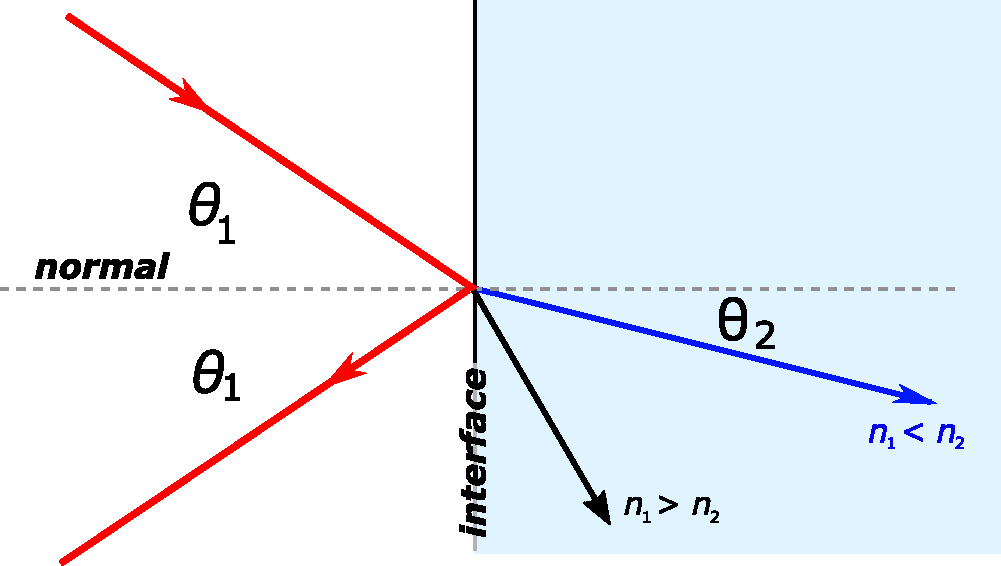
\includegraphics[scale=0.3]{david/index.pdf}
        \caption{Relación entre índice de refracción y el ángulo.}
    \end{figure}
\end{frame}
